\documentclass[conference]{IEEEtran}
\IEEEoverridecommandlockouts
% The preceding line is only needed to identify funding in the first footnote. If that is unneeded, please comment it out.
\usepackage{cite}
\usepackage{amsmath,amssymb,amsfonts}
\usepackage{algorithmic}
\usepackage{graphicx}
\usepackage{textcomp}
\usepackage{xcolor}

\usepackage{multirow}
\usepackage{rotating}

\usepackage{mdframed}
\usepackage{hyperref}
\usepackage{tikz}
\usepackage{makecell}
\usepackage{tcolorbox}
\usepackage{amsthm}
%\usepackage[english]{babel}
\usepackage{pifont} % checkmarks
%\theoremstyle{definition}
%\newtheorem{definition}{Definition}[section]


\usepackage{listings}
\lstset
{ 
    basicstyle=\footnotesize,
    numbers=left,
    stepnumber=1,
    xleftmargin=5.0ex,
}


%SCJ
\usepackage{subcaption}
\usepackage{array, multirow}
\usepackage{enumitem}


\def\BibTeX{{\rm B\kern-.05em{\sc i\kern-.025em b}\kern-.08em
    T\kern-.1667em\lower.7ex\hbox{E}\kern-.125emX}}
\begin{document}

%\IEEEpubid{978-1-6654-8356-8/22/\$31.00 ©2022 IEEE}
% @Sune:
% Found this suggestion: https://site.ieee.org/compel2018/ieee-copyright-notice/
% I have added it - you can see if it fulfills the requirements

%\IEEEoverridecommandlockouts
%\IEEEpubid{\makebox[\columnwidth]{978-1-6654-8356-8/22/\$31.00 ©2022 IEEE %\hfill} \hspace{\columnsep}\makebox[\columnwidth]{ }}
                                 %978-1-6654-8356-8/22/$31.00 ©2022 IEEE
% copyright notice added:
%\makeatletter
%\setlength{\footskip}{20pt} 
%\def\ps@IEEEtitlepagestyle{%
%  \def\@oddfoot{\mycopyrightnotice}%
%  \def\@evenfoot{}%
%}
%\def\mycopyrightnotice{%
%  {\footnotesize 978-1-6654-8356-8/22/\$31.00 ©2022 IEEE\hfill}% <--- Change here
%  \gdef\mycopyrightnotice{}% just in case
%}

      
\title{Adaptive Architectures: Designing an Industry 4.0 Prototype Based on Scientific Research\\}

\author{
    \IEEEauthorblockN{
        Joachim R Baumann\IEEEauthorrefmark{1},
        Phillip Nielsen\IEEEauthorrefmark{1},
        Sebastian Revsbech Christensen\IEEEauthorrefmark{1}, \\
        Simone Cosentino\IEEEauthorrefmark{1},
        Oskar Præstholm\IEEEauthorrefmark{1},
        Hans Askov\IEEEauthorrefmark{1}
    } \\
    \IEEEauthorblockA{
        University of Southern Denmark, SDU Software Engineering, Odense, Denmark \\
        Email: \IEEEauthorrefmark{1} \textnormal{\{jobau19,phnie19,sechr17,sicos23,ospra20, haask19\}}@student.sdu.dk
    }
}


%%%%

%\author{\IEEEauthorblockN{1\textsuperscript{st} Blinded for review}
%\IEEEauthorblockA{\textit{Blinded for review} \\
%\textit{Blinded for review}\\
%Blinded for review \\
%Blinded for review}
%\and
%\IEEEauthorblockN{2\textsuperscript{nd} Blinded for review}
%\IEEEauthorblockA{\textit{Blinded for review} \\
%\textit{Blinded for review}\\
%Blinded for review \\
%Blinded for review}
%\and
%\IEEEauthorblockN{3\textsuperscript{nd} Blinded for review}
%\IEEEauthorblockA{\textit{Blinded for review} \\
%\textit{Blinded for review}\\
%Blinded for review \\
%Blinded for review}
%}

%%%%
%\IEEEauthorblockN{2\textsuperscript{nd} Given Name Surname}
%\IEEEauthorblockA{\textit{dept. name of organization (of Aff.)} \\
%\textit{name of organization (of Aff.)}\\
%City, Country \\
%email address or ORCID}



\maketitle
\IEEEpubidadjcol
\begin{abstract}

This paper explores an Industry 4.0 (I4.0) ball pen production system, investigating the feasibility of existing technologies to meet key quality attributes (QAs): interoperability, availability, deployability, and scalability. Emphasizing system scalability, the study designs a prototype software solution inspired by recent scientific articles. The prototype, leveraging MQTT and Kafka brokers, achieves a balance between efficiency and robustness. By centralizing data through Kafka and utilizing MQTT for lightweight IoT devices, the system handles over 20 sensors, maintaining latency below 1 second. Promising for I4.0 production, the paper recommends future work to test additional quality attributes and system components.
%%%%%%%%%%%%%%%%%% Max 970 signs without space %%%%%%%%%%%%%%%%%%
% Intro

% Gab
    
% Aim 

% Method

% Results 

\end{abstract}

\begin{IEEEkeywords}
Ball pen production, Industry 4.0 production, I4.0 production, Quality attribute experiment, Cell based production
\end{IEEEkeywords}


% input stuff here
\section{Introduction and Motivation}
While older software-systems have established an industry standard for their architectural design patterns, the growing requirements for new systems make it increasingly harder to keep up. In order to adapt, scientific authors examine the different architectures and their impact on quality attributes. These scientific articles serve as an inspiration for system developers for their system designs. For new production environments like Industry 4.0 (I4.0) the adaptation of a standard architectural design patterns is ongoing. This study uses scientific articles to design a prototype software-solution for an industry 4.0 production. The research resulted in a prototype using a combination of MQTT and Kafka.


\section{Problem, research questions and Approach}

\label{sec:problem}
A ball pen manufacturer needs to create a fully automated production line, with the specified requirements of high availability and easy interoperability, to avoid unnecessary downtime. 
The company wants the software architecture to support potential growth in production, so the ability to add more cells must be supported. 
When a fault occurs within the system architecture it needs to respond automatically to maintain high availability. To facilitate early problem fixing, the system should be monitored, either by a separate system or internally. All the data collected through monitoring needs to be sent to a separate system, to be analyzed in order to optimize the production.  \\ 

\begin{enumerate}
    \item Which architectural patterns would best align with the system's quality attributes?
    \item Which tech stack could contribute positively towards the required quality attributes?
    \item Which framework should manage internal communication between subsystems?\\
\end{enumerate}

The following steps were taken to answer this paper's research questions: 
\\
\begin{enumerate}
    \item Analyse the problem, and set a scope
    \item Find related works and articles
    \item Review chosen articles
    \item Analyse article solutions
    \item Use cases and Quality attribute scenarios
    \item Design solution
    \item Prototyping and testing
\end{enumerate}

\section{Related work}
\label{sec:related_work}
This Section addresses existing contributions by examining similar experiments conducted, and existing standards in the I4.0 domain. 
In total, 4 papers are investigated.
\\ \\
Article \cite{Lasi2014} summarizes the evolution into the industry 4.0 system, and describes the fundamental concepts and goals for I4.0 systems. By localizing responsibilities throughout the system, it becomes possible to adapt faster, enabling quicker decision-making.
Encapsulating responsibilities to individual parts of the system, increases overall system interoperability and resource efficiency which allows the choice of different software for individual system parts. 
In principle, this should also increase modifiability and deployability, since each part of the system works independently and any updates or changes would only affect the singular part. 

By following these industry 4.0 principles and concepts, integration becomes possible and the production can make use of value-creation networks, which should allow for considerable optimization of processes and possibly gain insight into new aspects of revenue. With a dynamic production network, data can be collected throughout the whole product life cycle.



In \cite{torben21} a state-of-the-art production system developed for I4.0 systems has been proposed. The production system in the study focuses particularly on flexibility and adaptability in the production system and proposes a model to fulfill these quality attributes. The production system is built with a Microservice architecture, as the different subsystems are abstracted away by being dockerized. This causes the system to be adaptable and flexible, as small changes to the micro-services, in case the requirements change, can easily be deployed.  The subsystems then communicate through a message bus. The production line itself is built with a four-cell system, controlled by PLCs, that can function in multiple complex processes.
\\ \\
In \cite{torben20pilot} a pilot study of the interoperability quality attribute in a minimum viable product (MVP) of producing a drone has been analyzed. The setting of creating the drone is a modern state-of-the-art I4.0 laboratory, where multiple communication protocols and other assets, e.g. the cells in the production line, are required to work together to produce the product. Through an analysis of these assets communicating, it is concluded that the interoperability in I4.0 systems is still immature. This is because of a lack of various requirements of interoperability from the different assets, such as a lack of good documentation, missing external interfaces, and other communication technologies. The reason for this could be an apparent lack of understanding of the necessity of asset interoperability in an I4.0 context.


For insight into how an I4.0 system could be applied to actual production, article \cite{Liu2022} analyzes several other scientific articles on the topic. The article concludes with the creation of a prototype, with the purpose of testing the system architecture. The architecture for the prototype is based on a comprehensive literature review and gap analysis of industry 4.0 platforms.

\begin{figure*}[!ht]
    \centering
    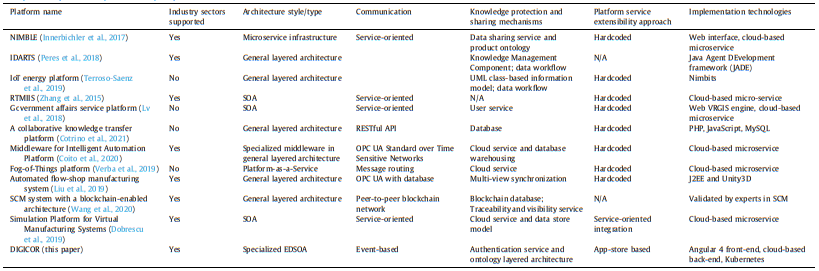
\includegraphics[scale=0.85]{Images/ArticleReviewRotate.png}
    \caption{Overview of system-architectures used for I4.0}
    \label{figure:1}
\end{figure*}


As seen in figure \ref{figure:1} from article \cite{Liu2022} the majority of the literature related to I4.0 uses different architectures, and an industry standard has not been formed. The article concludes that diverse quality attribute prioritization drives the different system architectures in different directions. After reviewing several of the different architectures, the authors decided that their system prototype's requirements aligned with either a micro-services or event-based architecture. In the end, when comparing the two, the event-based system allowed for higher performance, while keeping the interoperability aspect. The micro-service architecture added additional layers of complexity and fell behind in performance. In the end, the event-based architecture was decided for the prototype, as it had many of the perks of a micro-services architecture, while still maintaining a high performance.


\section{Use Case and Quality Attribute Scenario}
\label{sec:use_case_and_qas}
\noindent
This Section introduces the use case and the specified four QASes.
The QASes are developed based on the use case.
\\ \\
To facilitate an analysis of the needs of the ball pen manufacturer that is facing potential growth in their production, a use case analysis of the required system has been performed. The assumptions for creating the use cases are seen in table \ref{tab:Assumptions Table}.

\begin{table}[ht]
\centering
\begin{tabular}{|l|p{3.5cm}|p{3.5cm}|}
\hline
\textbf{ID} & \textbf{Assumption} & \textbf{Reasoning} \\
\hline
A1 & The pen consists of 5 parts & The disassembled pen shows this to be the case \\
\hline
A2 & 4 assembly steps are conducted by 4 individual cells & Minimum number of steps required to assemble the 5 parts of the pen. \\
\hline
A3 & Each cell contains sensors to monitor its own health and progress in its process. &  Sensor and monitor data need to be collected in order to operate the system. \\
\hline
A4 & Each cell has a box of parts that is fed into the assembly line to combine with the pen & The different cells need access to their respective parts. \\
\hline
A5 & Each cell monitors execution time, availability, performance, quality, and OEE & Data is needed to run diagnostics and perform optimization of the process. \\
\hline
A6 & Different cells may require software written in different languages. & For optimization and diagnostics. \\
\hline
A7 & The assembly line has to run without operator interaction (fully automated) & To reduce production times and labor costs. \\
\hline
A8 & A database should be used. & To store relevant data for logs. \\
\hline
A9 & The assembly line contains both parallel and sequential operations. & Some parts can be combined simultaneously, while the last part is dependent on two other cells. \\
\hline
A10 & The system uses pre-made parts therefore only assembly of the ball-pen is required. & The parts of the pen to be assembled are already made in a different area of production. \\
\hline
A11 & Quality control happens at each cell. & The sensors at the cells are able to conduct sufficient quality control. \\
\hline
\end{tabular}
\caption{Table of Assumptions and Reasoning}
\label{tab:Assumptions Table}
\end{table}

These assumptions were the basis for the use cases that are shown as in the following subsection \ref{sec:use_case}.

\subsection{Use case}
\label{sec:use_case}

Table \ref{tab:use-case-start-production} describes the process of starting the production system. The primary actor is the production manager who is responsible for initiating the process. The precondition of this is that he is logged into the software and that all the necessary materials, machine setups, and preliminary checks are ready. The main flow describes the production manager starting the production system and the subsequent steps this entails. The postcondition is that the system is operational. An alternative flow describes when the system diagnoses an issue.

\begin{table}[ht]
\centering
\begin{tabular}{|l|p{6cm}|}
\hline
\multicolumn{2}{|c|}{\textbf{Use Case: Start Production}} \\
\hline
\textbf{ID:} & U01 \\
\hline
\textbf{Primary Actor:} & Production manager \\
\hline
\textbf{Secondary Actor:} &  None \\
\hline
\textbf{Short Description:} & This process is responsible for the start of the production and the workflow connected to it. \\
\hline
\textbf{Preconditions:} & 
\begin{minipage}[t]{\linewidth}
\begin{itemize}
  \item The production manager, responsible for initiating production cycles, is logged into the software.
  \item All necessary materials, machine setups, and preliminary checks for production cells have been completed and are ready for operation.
\end{itemize}
\end{minipage} \\
\hline
\textbf{Main Flow:} & 
\begin{minipage}[t]{\linewidth}
\begin{enumerate}
  \item The production manager initiates the production via the central control software by clicking “start production”
  \item The production orchestrator conducts a status check for all cells, confirming the readiness for production.
  \item Upon successful status confirmation, each cell sends a ready signal back to the orchestrator.
  \item The control software notifies the production manager that the production has started.
  \item The user interface switches to display the production real-time status information screen.
\end{enumerate}
\end{minipage} \\
\hline
\textbf{Post conditions:} & 
\begin{minipage}[t]{\linewidth}
\begin{itemize}
    \item All production cells are operational, and the production manager is monitoring the system through a user interface.
\end{itemize}
\end{minipage}
\\
\hline
\textbf{Alternative Flow:} & 
\begin{minipage}[t]{\linewidth}
\begin{itemize}
  \item If the cells respond with a bad diagnostic, the production manager is notified, and the production start is canceled.
\end{itemize}
\end{minipage} \\
\hline
\end{tabular}
\caption{Use Case Specification for Starting Production}
\label{tab:use-case-start-production}
\end{table}

Table \ref{tab:use-case-error-diagnosis} is the use case for the process that happens to facilitate the error diagnostics of the system. The primary actor for this is again the production manager. The preconditions describe the conditions for the error diagnosis to take place. The main flow describes the steps the production manager must take to achieve this. The post-conditions indicate that the result of this is that an alarm has been activated, signaling the error. The alternative describes the case where the cells respond with a bad diagnosis, and the system can't handle it automatically.

\begin{table}[ht]
\centering
\begin{tabular}{|l|p{6cm}|}
\hline
\multicolumn{2}{|c|}{\textbf{Use Case: Error diagnosis}} \\
\hline
\textbf{ID:} & U02 \\
\hline
\textbf{Primary Actor:} & Production manager \\
\hline
\textbf{Secondary Actor:} &  None \\
\hline
\textbf{Short Description:} & This use case describes what happens to the system when an error has occurred. The production manager is logged into the system. \\
\hline
\textbf{Preconditions:} & 
\begin{minipage}[t]{\linewidth}
\begin{itemize}
  \item The production manager is logged into the centralized control system.
  \item An error has been detected in the production line, halting the production process.
\end{itemize}
\end{minipage} \\
\hline
\textbf{Main Flow:} & 
\begin{minipage}[t]{\linewidth}
\begin{enumerate}
  \item The production manager clicks “Error diagnosis”
  \item The production orchestrator checks status for each cell in the production.
  \item Each cell sends diagnostic information in return.
  \item The diagnostic data is displayed at UI.
  \item An alarm or notification begins.
\end{enumerate}
\end{minipage} \\
\hline
\textbf{Post conditions:} & An alarm has occurred. \\
\hline
\textbf{Alternative Flow:} & 
\begin{minipage}[t]{\linewidth}
\begin{itemize}
  \item If any of the cells respond with a bad diagnostic, the production manager is notified.
  \item The system triggers a diagnostic routine in order to identify the issue.
  \item If the issue cannot be handled automatically, the production is stopped until manual intervention is initiated.
\end{itemize}
\end{minipage} \\
\hline
\end{tabular}
\caption{Use Case Specification for Error Diagnosis}
\label{tab:use-case-error-diagnosis}
\end{table} 

Table \ref{tab:use-case-stop-production} outlines the criteria for halting production and explains the subsequent actions that occur once the production manager has initiated the "stop production" command in the orchestration software's user interface, which controls the system.

\begin{table}[ht]
\centering
\begin{tabular}{|l|p{6cm}|}
\hline
\multicolumn{2}{|c|}{\textbf{Use Case: Stop Production}} \\
\hline
\textbf{ID:} & U01 \\
\hline
\textbf{Primary Actor:} & Production manager \\
\hline
\textbf{Secondary Actor:} & None \\
\hline
\textbf{Short Description:} & This process is responsible for stopping the production and the workflow connected to it. \\
\hline
\textbf{Preconditions:} & 
\begin{minipage}[t]{\linewidth}
\begin{itemize}
  \item The product manager is logged into the software.
  \item The production is running.
\end{itemize}
\end{minipage} \\
\hline
\textbf{Main Flow:} & 
\begin{minipage}[t]{\linewidth}
\begin{enumerate}
  \item The production manager clicks “Stop Production” from the orchestration software user interface.
  \item The production orchestrator sends a stop production message to each cell.
  \item The software notifies the production manager that the production has been stopped.
\end{enumerate}
\end{minipage} \\
\hline
\textbf{Post conditions:} & The production has stopped and the production manager has confirmed the pause in operations. \\
\hline
\textbf{Alternative Flow:} & Not applicable \\
\hline
\end{tabular}
\caption{Use Case Specification for Stopping Production}
\label{tab:use-case-stop-production}
\end{table}

\subsection{Quality attribute scenarios}
\label{sec:qas}
Based on the use cases, four quality attributes (QA) are identified to achieve the system.
\begin{enumerate}
    \item Interoperability
    \item Availability
    \item Deployability
    \item Scalability
\end{enumerate} 
\textit{Interoperability} is important, as the multiple systems for production have to work together. The use cases show that the system contains various software and hardware components that need to work in unison. Interoperability ensures that this can happen. Data flow is also important, as seen in table \ref{tab:use-case-start-production} where the organizational system requires diagnostics of the cells, ensuring that they are operational to show the production manager that everything is operational in the user interface. The same is the case for \ref{tab:use-case-error-diagnosis} where error diagnostics of the cells require interoperability between the different systems to identify the issue. Interoperability is also part of ensuring scalability, as it allows for the integration of new technologies without interrupting the entire workflow. \\ \\
\textit{Availability} is important for a system such as this, as any downtime directly translates into lost productivity. It is also important as seen in the process flows in the table, where the production manager has to make informed decisions based on the feedback from the user interface in real-time. If any parts of the system are unavailable, this might be impossible. It is also directly tied to maintenance and upkeep, as these are also based on system feedback as seen in table \ref{tab:use-case-error-diagnosis}. If this is not available, this can have consequences for the equipment or the safety of the workers. \\

\textit{Deployability} allows the system to be easy to set up quickly and configure with minimal effort. Depending on the system, different deployability orchestrators may have an advantage over others. Deployability also denotes the system's recovery speed, ensuring that in case an issue is identified the system will quickly be able to recover, minimizing downtime. This is also a requirement for the system to gain maintenance, as the production demand grows the system can be scaled to accommodate the increased load. \\


\textit{Scalability} is important since the ball pen manufacturer is facing potential growth. A system with scalability will allow the manufacturer to scale up without any downtime in production. The system will also be able to handle the potential increase in error checks that have to be performed.

\section{The solution}
\label{sec:middleware_architecture}

% Description of the overall architecture designs
% Argue for tactics used to archieve the QASes
% Discuss the trade-offs

This section describes the design of a prototype, which will be used to test if the selected architecture supports the quality attributes.

The initial candidates for the architecture, based on the research articles from chapter \ref{sec:related_work}, pointed towards implementing the system in a micro-service pattern or an event-driven pattern.
The conclusion was to use a micro-service pattern for overall communication between each system and within the micro-service pattern, to implement the production system with the event-driven software architecture. 
By using an event-driven architecture for the conveyor belt and its sensors, the system becomes capable of sharing real-time data, while adapting to changes if necessary. via asynchronous communication. 
By using a message bus for communication, the individual parts can remain loosely coupled increasing the overall interoperability of the system, while the different system components, become individually scalable. The downside to using these architectural patterns is the increased complexity in implementation. While the architecture behind the conveyor belt does not require a lot of different components, if the production later needs to add additional features, the complexity could become problematic.
\\
The entire system consists of many individual services, ranging from log collection to an inventory management system. Each system contains several sub-systems with different purposes see figure \ref{figure:2}.
\begin{figure}[ht]
    \centering
    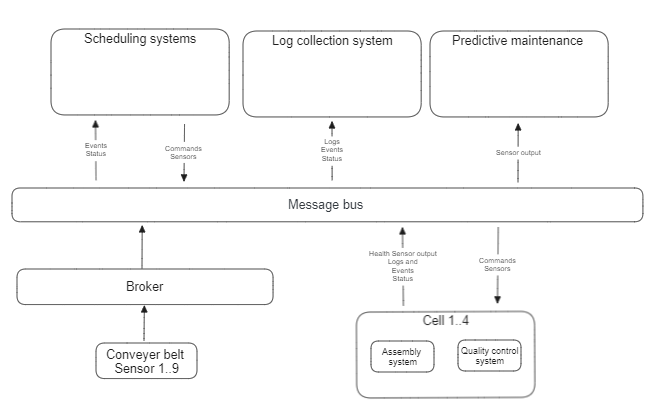
\includegraphics[scale=0.5]{Images/OverallArchitecture.png}
    \caption{The physical production layout}
    \label{figure:2}
\end{figure}


\
Designing the architecture as a whole and making design decisions for each system, would be too time-consuming and out of scope, considering the purpose is to create a testable prototype for an I4.0 production. 
As a result, the proposed solution will solely focus on the production system.

\subsection{Designing the production}
The physical production consists of 4 cells, each adding 1 additional part to the pen. Between these cells, there are sensors, which tell the next cell when the pen is ready. 
An illustration can be seen in figure \ref{figure:3}. Cells one and two operate in parallel while three and four operate sequentially as defined in \cite{torben21}.

\begin{figure}[ht]
    \centering
    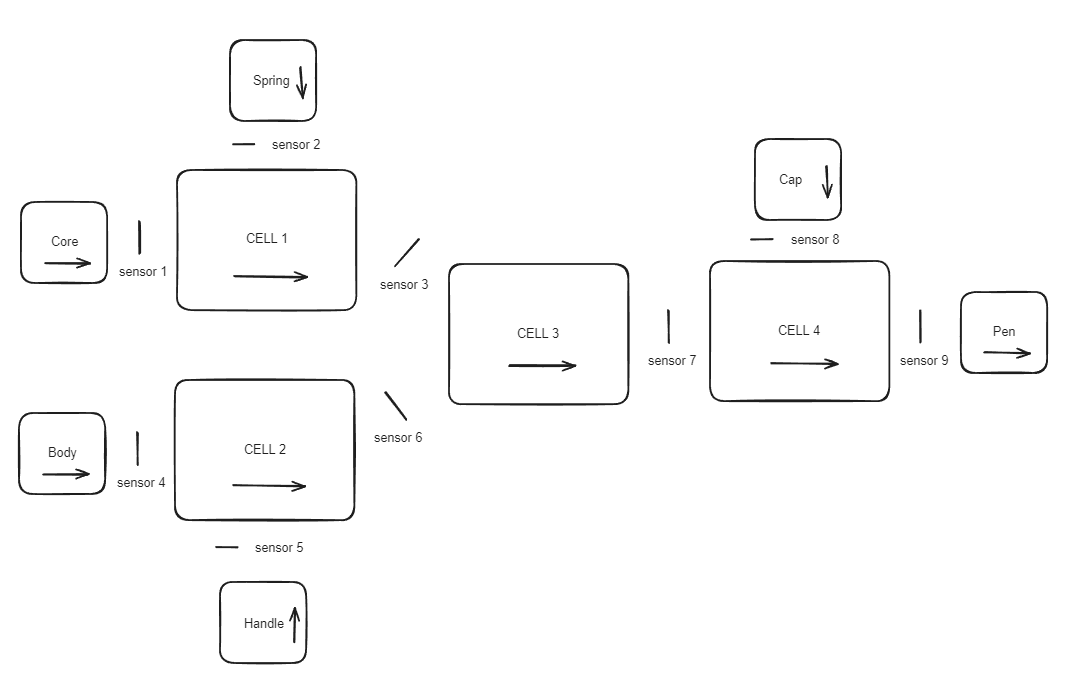
\includegraphics[scale=0.3]{Images/ProductionLayout.png}
    \caption{The physical production layout}
    \label{figure:3}
\end{figure}

Each cell contains a robotic system responsible for assembling or combining parts to create the pen. The cells contain several sensors ranging from when the pen is ready for further assembling to collecting health data, from the cell. By having sensors collecting health data frequently, it should become possible to predict maintenance and investigate why errors occur.
\
\subsubsection{Message Bus}
To manage this large quantity of data, the event-driven architecture becomes relevant. By implementing a message bus to manage the data flow within the system, each cell keeps its interoperability and stays individually scalable. \\ 
The message bus is responsible for receiving all the data from the different sensors and creating topics, where the relevant recipient can subscribe to receive the data.
For the production system, several MOMs (Message Oriented Middleware) were considered. According to \cite{Message-orientedMiddleware} the 4 most prominent within production systems are: 
MQTT, AMQP, and Kafka, which are all based on a broker, and ZeroMQ, which is brokerless. \\
Kafka has an edge over the others, due to the ability to replay messages:
“A unique approach having durable saved message streams and the ability to jump back and forth is taken by Kafka”\cite{Message-orientedMiddleware}. 
Kafka does this better than the other communication patterns while also allowing multiple publishers to write on the same topic.

Kafka is well-suited for real-time data streaming and event-driven architectures, while MQTT is tailored for lightweight, efficient communication in IoT scenarios. For that reason, each sensor between the cells will use the MQTT message bus to keep it lightweight and limit hardware usage. Kafka will mainly be responsible for handling the enterprise part of the system. 
However, a bridge/proxy between MQTT and Kafka will be created to analyze and save the data from the cells. 
Using both Kafka and MQTT collaboratively within the systems, allows the architecture to reap the benefits of both keeping the sensors lightweight, and having the Kafka capabilities for the rest of the system.
Working collaboratively with Kafka and MQTT has been implemented successfully before as seen in \cite{HiveMQTTvsKafka}.
While the sensors between cells will be communicating using the MQTT bridge, each individual cell will be transmitting its data directly to Kafka. 
\\
\subsubsection{Database Choice}
The production management system itself, will not have its own database, but the log data from the sensors still needs to be stored. This responsibility lies within the log collection system, which collects the data from Kafka via. an internal API. The data is then stored within a time series\cite{timeseries_db} database for later or ongoing analysis.
By storing this data the system becomes able to analyze itself in various ways. By continually checking the data sent from the sensors, it becomes possible to create a predictive model, which makes fault prevention possible. In the case a fault occurs, it should be detected quickly by monitoring the heartbeat continuously, through the data sent.


\section{Evaluation}
\label{sec:evaluation}
This Section describes the evaluation of the proposed design.
Section \ref{sec:design} introduces the design of the experiment to evaluate the system. 
Section \ref{sec:measurements} identifies the measurements in the system for the experiment.
Section \ref{sec:experiment_data} describes the pilot test used to compute the number of replications in the actual evaluation. 
Section \ref{sec:analysis} presents the analysis of the results from the experiment. 

 
\subsection{Experiment design}
This chapter describes in detail the testing done on the prototype designed in chapter \ref{sec:middleware_architecture}, to validate its ability to fulfil the quality attributes.\\
\label{sec:design}
This experiment is supposed to test the scalability quality attribute associated with the system architecture. To test this a prototype, mainly consisting of mocked sensor data, transmits the mocked data to Kafka through a MQTT broker. The Kafka message bus creates a topic, to which a subscriber created in Spring subscribes. The subscriber transmits the data to a Postgres database, where it is stored for analysis. All of this is managed by a docker-compose network.
By using docker-compose for the different services it becomes possible to scale based on demand, which is what this experiment is testing.
The purpose of the experiment is to test if Kafka can handle increased traffic load from the publisher, which sends the data. To achieve this, several publisher services are booted up at the same time.
By testing, if Kafka can handle additional stress from the publishers, we gain insight into the system's ability to scale, if the company wants to add additional cells and therefore more sensors to the production. \\
To determine if the architecture meets the requirements set for the quality attribute a hypothesis has been formed: \\
"The architecture will be able to maintain a transmission time below 2 seconds while transmitting data from up to 20 sensors" 

\subsection{Measurements}
\label{sec:measurements}

The command “docker-compose up” is used to initiate each test.
After having the system run for 4 minutes, the publisher services are manually closed through Docker desktop.
Within the subscriber-service a REST API has been created, which exports the data from the Postgres database to JSON format.
After formatting the data to csv, it is imported to Excel ready for analysis.
The part of the data of interest is the timestamp the publisher sends, which indicates when the sensor has picked up the data, and the timestamp the Postgres database creates once it lands in the database. By subtracting the publisher timestamp from the database timestamp, we’re able to calculate the ms it takes to transmit the data from the “sensor/publisher” to the database.


\newpage
\subsection{Experiment Data}
\label{sec:experiment_data}
After running the experiments accessing the endpoint that creates a JSON file, and converting that JSON file to csv format the data was assembled into a single csv file. Figure \ref{figure:4} shows a data example of this.
\begin{figure}[!ht]
    \centering
    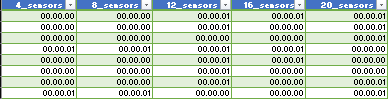
\includegraphics[scale=0.8]{Images/Data_sample.png}
    \caption{Small data sample}
    \label{figure:4}
\end{figure}

The data is stored as a time object, which goes dd(days)-hh(hours)--ss(seconds). In the example on \ref{figure:4} it can be seen that the largest transmission times hover around 1000 ms.



\subsection{Analysis}
\label{sec:analysis}
To gain an insight into all the data, each sensor's data was plotted to illustrate the differences and create a comparison.

\begin{figure}[!ht]
    \centering
    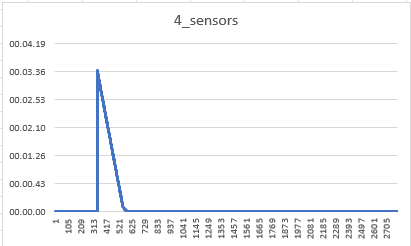
\includegraphics[scale=0.8]{Images/4sensors.png}
    \caption{4 sensors plotted}
    \label{figure:5}
\end{figure}

\begin{figure}[!ht]
    \centering
    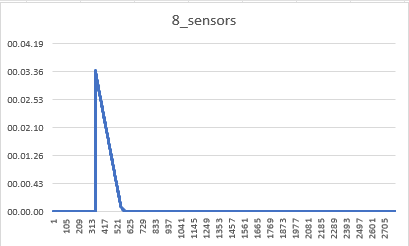
\includegraphics[scale=0.8]{Images/8sensors.png}
    \caption{8 sensors plotted}
    \label{figure:6}
\end{figure}

\begin{figure}[!ht]
    \centering
    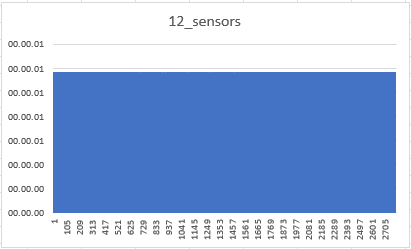
\includegraphics[scale=0.8]{Images/12sensors.png}
    \caption{12 sensors plotted}
    \label{figure:7}
\end{figure}

\begin{figure}[!ht]
    \centering
    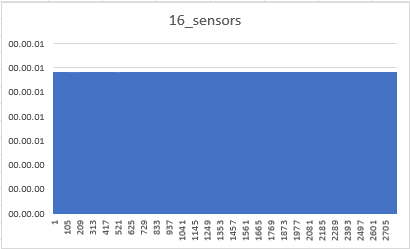
\includegraphics[scale=0.8]{Images/16sensors.png}
    \caption{16 sensors plotted}
    \label{figure:8}
\end{figure}

\begin{figure}[!ht]
    \centering
    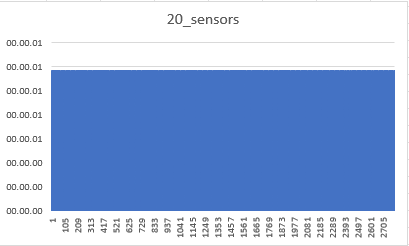
\includegraphics[scale=0.8]{Images/20sensors.png}
    \caption{20 sensors plotted}
    \label{figure:9}
\end{figure}

We can see on the graphs that sensors 4 (figure \ref{figure:5}) and 8 (figure \ref{figure:6}) tend to stay at sub 1000 ms transmission type, with similar outliers. When inspecting these outliers manually it can be seen that it is the first data sent to Kafka, which lingers until Kafka has established a connection to the database. Once the connection is established there is already live data flowing through the system, so Kafka stores the data, and sends it once the live data stream either pauses or is stopped. This results in a few outliers, matching up with the lifetime of the system during the experiment.
Once the test has 12+ sensors, the amount of data sent through the system increases, because of this, and to keep the data comparable the data was limited to 3000 samples from each test. By removing data from the past 3000 samples, the data that would have had an extended lifetime in the system from the experiments with 12, 16, and 20, does not display in the graphs.
By looking past the outliers it can be concluded that the data stays below 1s response time when scaled from 4 to 20 sensors. This means the system architecture allows scaling of producers within the system, and therefore by extension allows the addition of several cells to the system and confirms the hypothesis.
\section{Future work}

With the current prototype setup, the only load on Kafka is through the sensors, mocked with the producer service. To reach a state where it can be confidently concluded that the software architecture is viable to support the production of the I4.0 standard, further parts of the system would have to be mocked. By mocking more systems it would be easier to tell if Kafka could maintain a low ms on the data transmissions while supporting a complete production architecture.
Other quality attributes than scalability should also be tested, more specifically the availability and deployability attributes.
With the current prototype, the system is handled within docker-compose, which has sole responsibility for the deployability. It could be very interesting to compare the capabilities of docker-compose and an alternative like Kubernetes.
While testing the scalability of Kafka, the system had an increasingly higher load each time it was booted up. To test the availability it would be a good idea to do live load testing and stress testing, where the system gets gradual increases or even major spikes in data traffic to see the response. 
\section{Conclusion}

In conclusion, our exploration into the ball pen production system has made strides toward a more intelligent and efficient manufacturing approach. Drawing inspiration from key literature, especially \cite{Liu2022}, we crafted a prototype that blends Kafka and MQTT technologies. This strategic combination ensures our system functions smoothly with small sensors while offering scalability to handle increased data demands.
The pivotal scalability test gauged the system's capability to manage heightened workloads with the addition of more production elements. Encouragingly, our prototype demonstrated the ability to maintain data transmission times below 1000 milliseconds, even with the integration of twenty sensors. This success not only affirms the system's adaptability for accommodating additional production cells but also positions us for future developments.
Nevertheless, it's crucial to acknowledge that our current prototype, while showing promise in scalability, remains in its early stages. Further refinements are necessary, including simulating additional system components, scrutinizing attributes related to availability and deployability, and conducting more in-depth testing under realistic workloads.
Our endeavor transcends academic pursuits, aiming to contribute to the evolution of manufacturing processes by infusing intelligence and adaptability. This project serves as a foundational step for ongoing exploration and advancements in manufacturing. Envisioning a future where manufacturing processes are not just intelligent but continually improving, we anticipate the unfolding paradigm shift in adaptable and efficient production systems aligned with Industry 4.0.
In summary, the presented prototype and its evaluation substantiate the viability of the proposed system architecture, representing a key advancement toward intelligent and scalable manufacturing processes. This work provides insights into the future landscape of manufacturing, fostering a pathway for the integration of smart and dynamic production systems that align with the requirements of Industry 4.0.
\cite{Liu2022}

\newpage

\bibliographystyle{IEEEtran}
\bibliography{references}
\vspace{12pt}
\end{document}
